\section{The coordinate structure of the forest}\label{sec:forest}

We first establish the structural facts needed to separate a vector
into finitely many coordinates and its complement. The finite heights
give reflexivity and coordinate density; the ancestral order gives
contractive projections and an exact norm formula on the complementary
subtrees.

For a finite set $H$, the coordinate projections are
$P_Hu=\sum_{v\in H}u(v)e_v$ on $J$ and
$P_Hx=\sum_{v\in H}x(e_v)e_v^*$ on $X$; write $Q_H=I-P_H$.

\begin{lemma}\label{lem:forest-structure}
The space $X$ defined by \eqref{eq:segment-norm} is infinite dimensional,
separable, and reflexive, and the coordinate functionals have dense span
in $X$. Let $H\subset\mathcal F$ be finite and \emph{ancestral}, meaning
that it contains every ancestor of each of its vertices. The coordinate
projections $P_H$ and $Q_H$ are contractive on both $J$ and $X$.
Moreover, $P_Hx\to x$ along any increasing ancestral exhaustion of
$\mathcal F$.
\end{lemma}

\begin{proof}
Singleton tests give $\|u\|_2\le\rho(u)$. On a component of height
$h$, each segment has at most $h+1$ vertices. Thus Cauchy--Schwarz and
disjointness give
\[
 \|u\|_2\le\rho(u)\le\sqrt{h+1}\|u\|_2.
\]
Write $J_h$ for the completion on that component. Segment families
from different components combine freely, so
\[
 J=\left(\bigoplus_{h\ge1}J_h\right)_{\ell_2}.
\]
Each $J_h$ is isomorphic to Hilbert space. The dual of an $\ell_2$
sum is isometrically the $\ell_2$ sum of the duals: Cauchy--Schwarz
proves one inequality, and testing on almost norming unit vectors in
finitely many components, with proportional weights, proves the other.
Applying this identity twice proves reflexivity. In particular $X^*=J$
canonically. If the coordinate functionals did not have dense span in
$X$, Hahn--Banach would give a nonzero element of $X^*=J$ annihilating
them. All its coordinates would vanish, a contradiction. Countability
of $\mathcal F$ now proves separability; the independent coordinates
prove infinite dimensionality.

A segment meets $H$ in a prefix and its complement in a suffix.
Restricting disjoint segment tests to either set therefore proves
contractivity on $J$. The adjoints give precisely the coordinate
projections on $X$, and remain contractive. Finally, approximate $x$
by a finite coordinate combination. Once $H$ contains its support,
contractivity bounds the discarded tail of $x$ by that approximation
error. This proves convergence along an ancestral exhaustion.
\end{proof}

In particular, the completion of the finite coordinate functionals in
\[
 \|x\|=\sup\left\{\sum_vx(v)u(v):u\in c_{00}(\mathcal F),\ \rho(u)\le1\right\}
\]
is exactly $X$, under the coordinate pairing. This identifies the dual
and coordinate-completion descriptions of the present finite-height
forest. Each component has infinitely many vertices; only its height
is finite, and no Hilbert equivalence constant uniform in the height
was needed.

For $x=P_Hx$, restriction to $P_HJ$ preserves its functional norm.
The finite-dimensional unit ball is compact, so there is $f=P_Hf$
with $\rho(f)\le1$ and $x(f)=\|x\|$. If $x\ne0$ then $\rho(f)=1$;
if $x=0$, including when $H$ is empty, take $f=0$.


Let $G_H$ be the set of minimal vertices outside $H$. We call these
vertices \emph{gates}. They include roots of components disjoint from
$H$. Distinct gates are incomparable, and the descendant sets
$U_g=\{v:g\preceq v\}$ partition $\mathcal F\setminus H$.
Each segment crossing from $H$ to its complement passes through one
gate. Figure~\ref{fig:forest-gates} illustrates the partition.
\begin{figure}[ht]
\centering
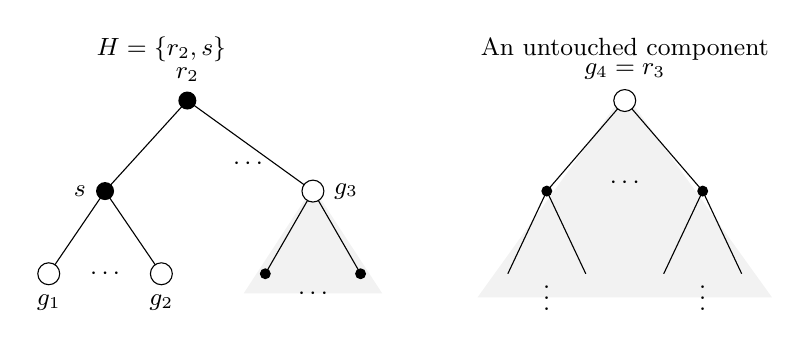
\begin{tikzpicture}[x=1.1cm,y=1cm,
 head/.style={circle,fill=black,inner sep=2.3pt},
 gate/.style={circle,draw,fill=white,inner sep=2.8pt},
 vertex/.style={circle,fill=black,inner sep=1.4pt},font=\small]
\fill[black!5] (1.4,1.1)--(.6,-.25)--(2.2,-.25)--cycle;
\fill[black!5] (5,2.3)--(3.3,-.3)--(6.7,-.3)--cycle;
\draw (-.05,2.2)--(-1,1.05)--(-1.65,0);
\draw (-1,1.05)--(-.35,0);
\draw (-.05,2.2)--(1.4,1.05);
\draw (1.4,1.05)--(.85,0);
\draw (1.4,1.05)--(1.95,0);
\node[head,label=above:$r_2$] at (-.05,2.2) {};
\node[head,label=left:$s$] at (-1,1.05) {};
\node[gate,label=below:$g_1$] at (-1.65,0) {};
\node[gate,label=below:$g_2$] at (-.35,0) {};
\node[gate,label=right:$g_3$] at (1.4,1.05) {};
\node[vertex] at (.85,0) {};
\node[vertex] at (1.95,0) {};
\node at (-1,.0) {$\cdots$};
\node at (.65,1.4) {$\cdots$};
\node at (1.4,-.25) {$\cdots$};
\node at (-.35,2.85) {$H=\{r_2,s\}$};
\draw (5,2.2)--(4.1,1.05)--(3.65,0);
\draw (4.1,1.05)--(4.55,0);
\draw (5,2.2)--(5.9,1.05)--(5.45,0);
\draw (5.9,1.05)--(6.35,0);
\node[gate,label=above:{$g_4=r_3$}] at (5,2.2) {};
\node[vertex] at (4.1,1.05) {};
\node[vertex] at (5.9,1.05) {};
\node at (5,1.15) {$\cdots$};
\node at (4.1,-.2) {$\vdots$};
\node at (5.9,-.2) {$\vdots$};
\node at (5,2.85) {An untouched component};
\end{tikzpicture}
\caption{A finite ancestor-closed head and some of its gates.  Black
large nodes belong to $H$; circled nodes are gates.  Shading indicates
two complementary descendant cones.  Only finitely many of the
countably many branches are drawn.  In particular an untouched
component begins with a gate at its root.}\label{fig:forest-gates}
\end{figure}

 Let $J(U_g)$ denote the coordinate subspace of $J$ supported in
$U_g$, with its inherited norm.

\begin{lemma}\label{lem:cones}
For every finite ancestral $H$,
\begin{equation}\label{eq:cone-decomposition}
 Q_HJ=\left(\bigoplus_{g\in G_H}J(U_g)\right)_{\ell_2},
 \qquad
 \|Q_Hx\|^2=\sum_{g\in G_H}\|x|_{J(U_g)}\|^2\quad(x\in X).
\end{equation}
The gate-coordinate map $x\mapsto(x(e_g))_{g\in G_H}$ is a contraction
from $X$ to $\ell_2(G_H)$.
\end{lemma}

\begin{proof}
On a vector supported outside $H$, every segment test reduces to a
segment in one cone. Grouping a disjoint family by its gates gives the
upper estimate for the first identity; combining almost maximizing
families from finitely many distinct cones gives the reverse estimate.
Pass to the completion. A functional supported outside $H$ has exactly
the norm of its restriction to $Q_HJ$, because $Q_H$ is contractive.
Duality for the $\ell_2$ sum therefore proves the second identity.

A segment contains at most one gate, so $\rho(u)=\|u\|_2$ for
vectors supported on $G_H$. Testing $x$ on such finite vectors proves
the gate-coordinate contraction.
\end{proof}

If $A$ is any antichain and $(a_v)_{v\in A}$ has finite support, then
\begin{equation}\label{eq:antichain-isometry}
 \rho\left(\sum_{v\in A}a_ve_v\right)
 =\left\|\sum_{v\in A}a_ve_v^*\right\|
 =\left(\sum_{v\in A}a_v^2\right)^{1/2}.
\end{equation}
The first equality with the Euclidean norm follows because a segment
meets $A$ at most once. For the dual norm, singleton tests give the upper
bound, and testing on the proportional vector supported on $A$ gives
the lower bound. Thus these identities concern the specified norm,
not merely equivalent norms on the same coordinate space.
